\section{Structure of CBF PDF Reports}
\label{sec:report_structure}

Figure~\ref{fig:report_example} shows an example of a match report from the 2013 season between CR Vasco da Gama and Associação Portuguesa de Desportos.
This example illustrates how the report is structured and helps understand how the principal information can be extracted.

\begin{figure}[htbp]
    \centering
    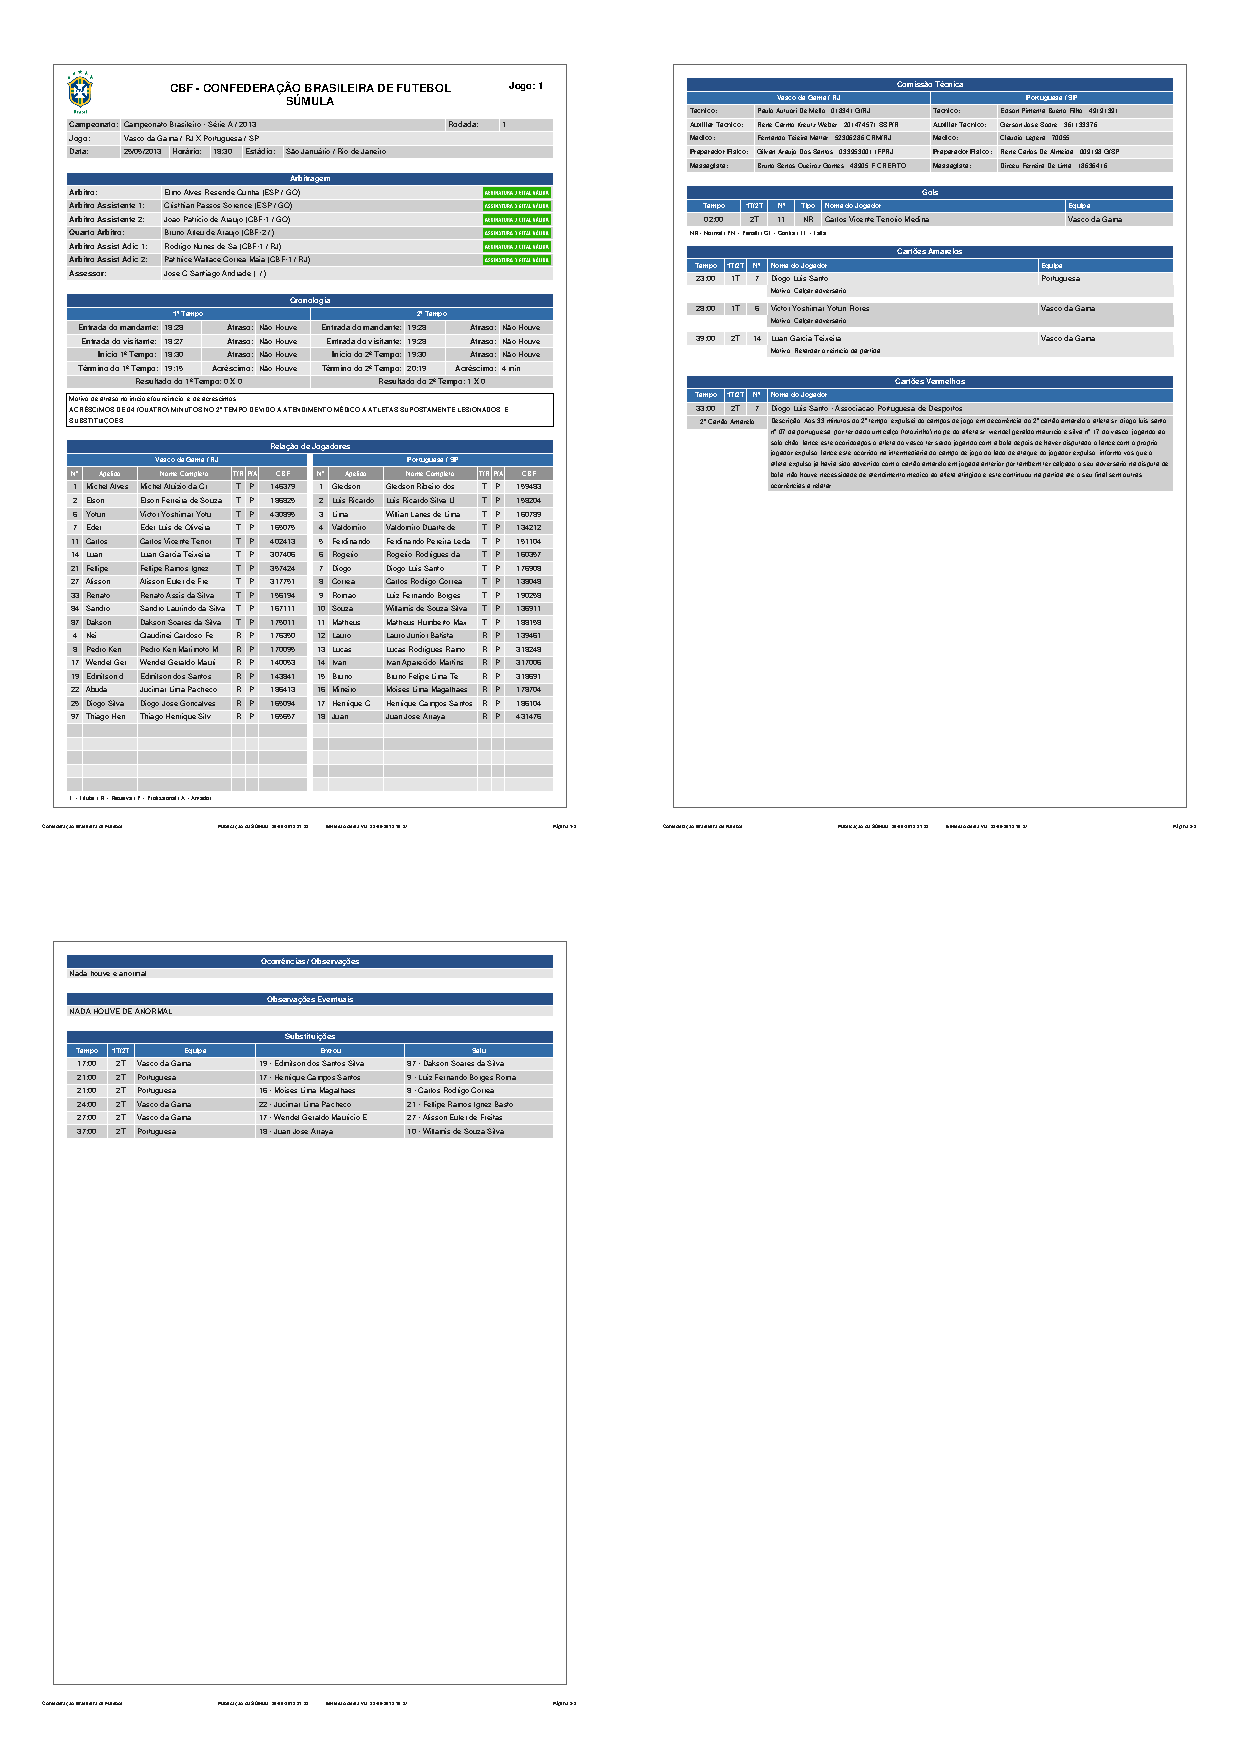
\includegraphics[width=0.9\textwidth]{figures/report.pdf}
    \caption{
        \textbf{Example of a CBF match report}.
        Example report from a match between CR Vasco da Gama and Associação Portuguesa de Desportos, which took place on May 25th, 2013, for the first round of the Brazilian First Division (\textit{Série A}).
    }
    \label{fig:report_example}
\end{figure}

The report begins with a header containing match details: championship, round, game, date, time, and stadium.
Then, we have the referee information, followed by the chronological details of the game.

Next, we have the player line-up relation as two tables, one for each club.
For each player, the table includes their jersey number, nickname, and full name.
Players in the starting line-up are marked with a ``T'', while substitutes are marked with a ``R''.
The table also indicates whether each player is professional (P) or amateur (A).
Each player is identified by their unique CBF id, which we use internally throughout our data extraction and processing workflow instead of player names, since names are more sensitive to encoding issues and may have inconsistent accentuation across reports.
Following the players' relation we have information on the coaching and medical staff.

After the team information, the report contains data on the events that occurred during the match.
This section starts with the goals scored during the match.
The report saves this information on two columns for time because in Brazil the game is divided and counted in two periods with 45 minutes each.
In this sense, unlike other countries, the minute 65 of a game is assigned as 20 minutes of the second period.
For each goal, the table includes when it was scored (minute and period), the scorer's jersey number and name, the type of goal, which can be open-play (NR), penalty (PN), own goal (CT), or free kick (FT), and the club for which the goal counts.

Yellow and red card data is found right after the goal data.
The first section is related to yellow cards, while the second is to red cards.
The organization of these sections follows the same structure as the goals table, except that the goal type field is not applicable.
For each card, the table includes when it was shown (minute and period), the player's jersey number and name.
An extra field, right below the player's name, indicates the reason for the card, though this information is not extracted in our retrieval process.

After these sections, we have substitution information.
This section is also organized as a table.
For each substitution, the table includes when it was made (minute and period), which club made the substitution, and the jersey number and full name of both the player entering and the player exiting the field.

At the end of the report, we have two sections for any occurrence or observation that the referees' team thinks is relevant.
